\section{Fourier Series}
%-----------------Orthonormal functions--------------------%
\subsection{Orthonormal Functions}
\begin{itemize}
\item \textbf{Orthonormal functions} has the following property:
\[ \langle \phi_{i}(t), \phi_{k}(t) \rangle = \begin{cases}
0, & i \neq k\\
1, & i = k\\
\end{cases} \]
The $N$ signals $\{ \phi_{i}(t)\}_{i=1...N}$ with this property is referred to as an \textbf{orthonormal set of signals}.\\\\
\textit{Think the orthogonal unitary vectors defining coordinate axes ($i,j,k$) in Euclidean space!}

\item Consider a generic signal that can be described by a \textbf{linear combination} of a set of orthonormal signals:
\[ x(t) = \sum_{i=1}^{N} a_{i} \phi_{i}(t) \]
where $a_{i}$ are unknown complex or real numbers. %, can be described as $\vec{A}=A_{x}\vec{i}+A_{y}\vec{j}+A_{z}\vec{k}$
\item The coefficients $a_{i}$ can be determined by projecting the signal into each function $\{ \phi_{i}(t)\}_{i=1...N} $:
\begin{align*}\begin{split}
\langle x(t), \phi_{k}(t) \rangle  &= \langle \sum_{i=1}^{N} a_{i} \phi_{i}(t), \phi_{k}(t) \rangle \\
&= \int_{-\infty}^{\infty} \sum_{i=1}^{N} a_{i} \ \phi_{i}(t) \ \phi_{k}^{*}(t) dt\\
&=\sum_{i=1}^{N} a_{i} \int_{-\infty}^{\infty}\phi_{i}(t) \ \phi_{k}^{*}(t) dt \\
&=a_{k}
\end{split} \end{align*}
% for $k= 1,2,3,...,N$.
 \begin{itemize}
 \item Scalar product is a linear operator.
 \item The coefficients provide all the information in the signal: if we know $a_{k}$, we know the signal.
 \item If the signal $x(t)$ belongs to a larger space, the projected signal will be an \textit{approximation} of the original signal with minimum MSE.
 \end{itemize} \end{itemize}

\begin{ex}{- Haar basis function}
Given the signal:
\[ \psi(t) = 
\begin{cases}
    1,      &   0 \leq t < \frac{1}{2}\\
    -1,     &   \frac{1}{2} < t \leq 1\\
    0,      &   \text{otherwise}\\
\end{cases} \]
The following signals define a set of orthonormal basis functions:
\[ 
    \psi_{rk} = \psi(2^{r}t-k) \ \text{for} \ r=0,1,2... \ \text{and} \ k=0,1,2,...,2^{r}-1 
\]

 \begin{figure}[H]
     \centering
     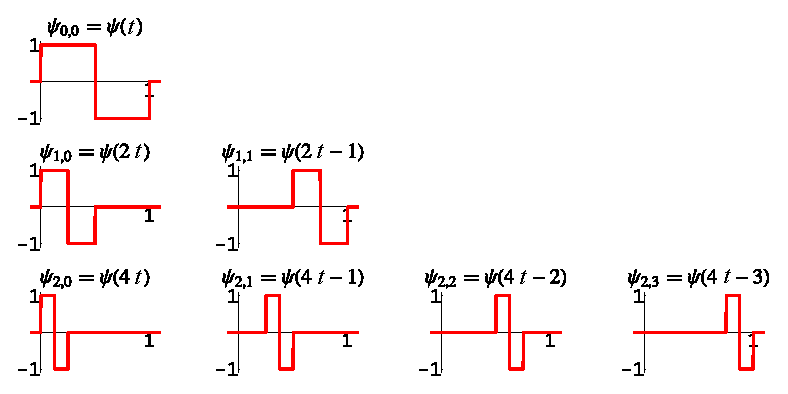
\includegraphics[width = \textwidth]{images/Haar_func.eps}
     \caption{Haar basis functions} 
 \end{figure}
\end{ex}
%-----------------Fourier basis functions--------------------%
\subsection{Fourier Basis Functions}
%A set of signals can be used to describe all signals in a given space of signals is called \textbf{s set of basis functions for that space}. They can be used to describe all other signals as linear combinations.

Fourier basis functions are:
\[ \phi_{i}(t) = \frac{1}{\sqrt{T}} e^{j\omega_{i} t} =  \frac{1}{\sqrt{T}} e^{j\frac{2\pi i}{T} t} \]
\ $t$ is defined in the time interval $[0,T]$.\\\\
These functions have the following properties:
\begin{itemize}
 \item periodic, $period = \frac{T}{i}$
 \item period is a function of the fundamental period $T$
 \item frequencies are the multiples of fundamental frequency $\frac{1}{T}$
 \item orthonormal, when $0 \leq t \leq T$:
 \begin{itemize}
   \item $i \neq k$,  \[ \langle \phi_{i}(t), \phi_{k}(t) \rangle = \int_{0}^{T}  \phi_{i}(t) \ \phi_{k}^{*}(t) dt = \frac{1}{T} \int_{0}^{T} e^{j\frac{2\pi i}{T} t}e^{-j\frac{2\pi k}{T} t} dt = 0\]
   \item $i=k$, \[ \langle \phi_{i}(t), \phi_{k}(t) \rangle  = \int_{0}^{T} \lvert \phi_{i}(t) \rvert^{2}dt = \frac{1}{T} \int_{0}^{T}dt =1\]
\end{itemize} \end{itemize}

%-----------------Fourier Series-------------------%
\subsection{Fourier Series}
\textbf{Fourier series}: can be used to represent any periodic signal with finite energy in a single period. 
\[ x(t) =  \sum_{k=-\infty}^{\infty} \ c_{k} \ e^{j\frac{2\pi k}{T}t} \quad \text{with} \quad c_{k} = \frac{1}{T} \int_{-\frac{T}{2}}^{+\frac{T}{2}} x(t)e^{-j\frac{2\pi k}{T}t} \]


\begin{dv}{}
If we assume:
\begin{align*}\begin{split}
 x(t) &= \sum_{i=-\infty}^{+\infty} \ a_{i} \ \phi_{i}(t) \\
&= \frac{1}{\sqrt{T}} \sum_{k=-\infty}^{+\infty} a_{k} \ e^{j\frac{2\pi k}{T}t}
\end{split} \end{align*}
with the coefficients $a_{k}$ :
\begin{align*}\begin{split}
a_{k} = \langle x(t), \phi_{k}(t) \rangle &=  \int_{0}^{T} x(t)\ \phi_{k}^{*}(t)dt \\
&=  \frac{1}{\sqrt{T}} \int_{0}^{T} x(t)\ e^{-j\frac{2\pi k}{T}t} dt 
\end{split} \end{align*}
An equivalent expression is the \textbf{Fourier series}
\[ x(t) =  \sum_{k=-\infty}^{+\infty} \ c_{k} \ e^{j\frac{2\pi k}{T}t} \quad \text{with} \ c_{k} = \frac{1}{T} \int_{0}^{T} x(t)e^{-j\frac{2\pi k}{T}t} dt \]
\end{dv}

\begin{itemize}
    \item The infinite set of orthonormal functions of the Fourier series describes any periodic signal with finite energy in a single period.
\end{itemize}

\begin{tcolorbox}[breakable]
Fourier series with a finite number of terms:
\[ x(t) \approx x_{N}(t) = \sum_{k=-N}^{+N} c_{k} e^{j\frac{2\pi k}{T}t} \]
Error of approximation decreases as the number of terms increases,
\[ E_{N}(t) = x(t)-x_{N}(t) = x(t)- \sum_{k=-N}^{+N} c_{k} \ e^{j\frac{2\pi k}{T}t} \]
\[ \lim_{N \to \infty} \int_{0}^{T} \lvert E_{N}(t) \rvert^{2} dt = 0, \quad \text{if} \ \int_{0}^{T} \lvert x(t) \rvert^{2} dt < \infty \] 
Fourier series converges as the number of terms increases:
\begin{figure}[H]
    \centering
    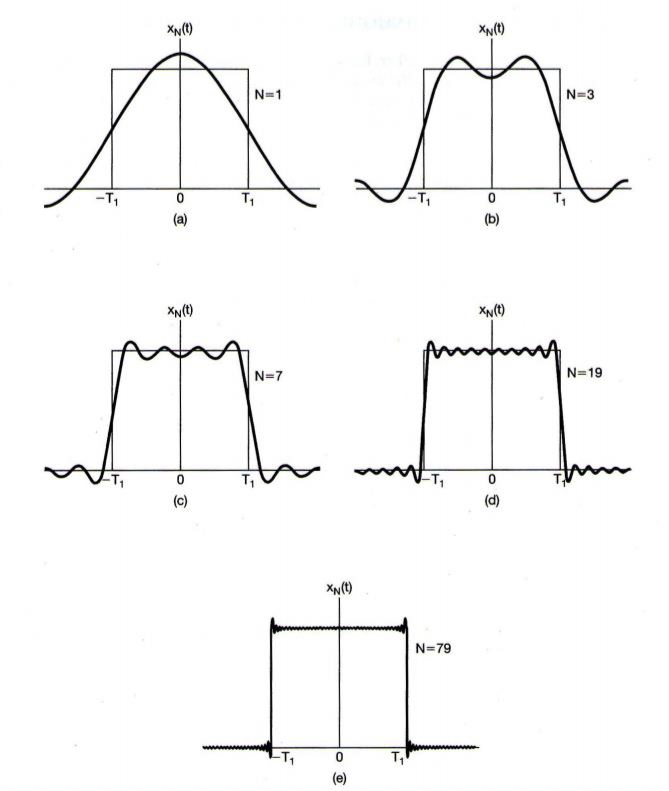
\includegraphics[width = 0.6\textwidth]{images/convergence}
    \caption{Example of convergence of the Fourier series of a periodic square wave} 
\end{figure}
\end{tcolorbox}
